\documentclass[tikz,border=10pt]{standalone}
\usepackage[dvipsnames]{xcolor}
\usepackage{tikz}

\usetikzlibrary{backgrounds}
\usetikzlibrary{calc}
\usetikzlibrary{fit}
\usetikzlibrary{positioning}
\usetikzlibrary{math}
\usetikzlibrary{trees}
\begin{document}

\centering
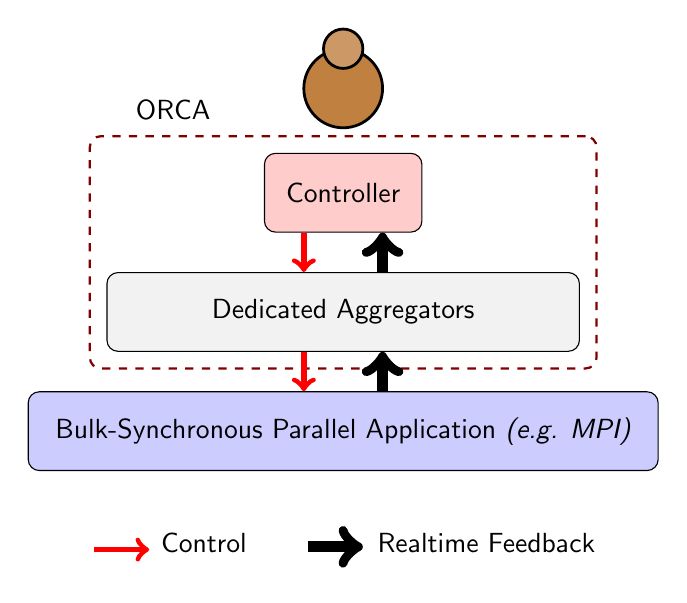
\begin{tikzpicture}[
		every node/.style={font=\sffamily},
		box/.style={draw, rounded corners=4pt, minimum width=2cm, minimum height=1cm, align=center},
		ctlarrow/.style={draw=red, line width=2pt},
		aggarrow/.style={draw, line width=4pt}
	]

	% Human figure
	\node[circle, draw=black, line width=1pt, fill=brown, minimum size=1cm] (body) {};
	\node[circle, draw=black, line width=1pt, fill=brown!80, minimum size=0.5cm, above=-8pt of body] (head) {};

	% CTL, AGG, MPI
	\node[box, fill=red!20, below=0.3cm of body] (ctl) {Controller};
	\node[box, fill=gray!10, below=0.5cm of ctl, minimum width=6cm] (agg) {Dedicated Aggregators};
	\node[box, fill=blue!20, below=0.5cm of agg, minimum width=8cm] (bsp)
	{Bulk-Synchronous Parallel Application \emph{(e.g. MPI)}};

	%\draw (ctl.north west) rectangle (agg.south east);
	%\draw ([x=agg.west, y=ctl.north west]) rectangle (agg.south east);
	%\draw[inner sep=6pt] (agg.west |- ctl.north west) rectangle (agg.south east);
	\node[
		draw=red!50!black,
		thick,
		dashed,
		rounded corners,
		inner sep=6pt,       % how much larger
		fit={(agg.west |- ctl.north west) (agg.south east)},
		label={[label distance=3pt]above left:ORCA}
	] {};

	% Arrows
	\draw[<-, aggarrow] ([xshift=0.5cm]ctl.south) -- ([xshift=0.5cm]agg.north);
	\draw[->, ctlarrow] ([xshift=-0.5cm]ctl.south) -- ([xshift=-0.5cm]agg.north);
	\draw[<-, aggarrow] ([xshift=0.5cm]agg.south) -- ([xshift=0.5cm]bsp.north);
	\draw[->, ctlarrow] ([xshift=-0.5cm]agg.south) -- ([xshift=-0.5cm]bsp.north);

	% Draw a legend box with "Control" and "Aggregation" texts next to their arrows
	%\begin{scope}[xshift=0cm, yshift=-8cm]
	\matrix[
		draw=white,
		rounded corners=2pt,
		fill=white,
		inner sep=4pt,
		column sep=12pt,
		anchor=north west,
		below=0.5cm of bsp.south
	] (legend) {
		\node[right] {\tikz \draw[->, ctlarrow] (0,0.1)--(0.7cm,0.1cm); Control}; &
		\node[right] {\tikz \draw[->, aggarrow] (0,0)--(0.7cm,0); Realtime~Feedback}; \\
	};
	%\end{scope}

\end{tikzpicture}

\end{document}
